\documentclass[a4paper]{article}

%% Language and font encodings
\usepackage[T1]{fontenc}
\usepackage[utf8x]{inputenc}
\usepackage[english]{babel}

\usepackage[colorlinks=true, allcolors=blue]{hyperref}

\urlstyle{tt}

\usepackage[sfdefault,lf]{carlito}
%% The 'lf' option for lining figures
%% The 'sfdefault' option to make the base font sans serif
\usepackage[parfill]{parskip}
\usepackage{float}
\renewcommand*\oldstylenums[1]{\carlitoOsF #1}
\usepackage{fancyhdr}
\usepackage{natbib}
\usepackage{authblk}
\setlength{\headheight}{41pt}

%% Sets page size and margins
\usepackage[a4paper,top=3cm,bottom=2cm,left=3cm,right=3cm,marginparwidth=1.75cm]{geometry}

%% Useful packages
\usepackage{amsmath}
\usepackage{amsfonts}
\usepackage{graphicx}
\usepackage{booktabs}

\usepackage[colorinlistoftodos]{todonotes}

%\renewcommand{\headrulewidth}{0pt}
\fancyhead[L]{\today}
\pagestyle{plain}
\title{Underwater Image Enhancement}
\author[1]{Arkadip Bhattacharya}
\author[2]{Arunangshu Biswas}
\author[3]{Pranjal Gain}
\author[+]{Dr. Abul Hasnat}
\affil[+]{Guide, Assistant Professor}
\affil[1,2,3]{Government College of Engineering and Textile Technology, Berhampore}

\setlength {\marginparwidth }{2cm}
\begin{document}
\maketitle
\thispagestyle{fancy}

\begin{abstract}
In this report, we present an approach for real-time underwater image enhancement using Cycle Generative Adversarial Network, or \textit{CycleGan}. The objective is to train the model to learn the mapping between the underwater image and the enhanced image using a training set of aligned image pairs. For the training we used the \textbf{EUVP} (Enhancing Underwater Visual Perception) a large scale dataset of a paired and an unpaired collection of underwater images (of ‘poor’ and ‘good’ quality) that are captured using seven different cameras over various visibility conditions during oceanic explorations and human-robot collaborative experiments. For our case, we have only supplied the images in an unpaired manner during the training for better generalisation of the mapping. The model and associated training pipelines are available at \url{https://github.com/darkmatter18/Underwater-image-enhancement}.
\end{abstract}

\section{Introduction}
\textit{Underwater optical imaging (OPI)} is a challenging field in computer vision research. Due to the medium, scattering always causes a blurring effect in underwater photography. The wavelength absorption usually causes a colour reduction in the captured images as well. In the shallow ocean, sunshine causes flickering effects. This causes the captured images with strong highlights. Whereas, the usage of artificial lighting for underwater photography causes vignetting in captured images due to the non-uniform nature of the lighting. Common issues with underwater images, such as light attenuation, scattering, non-uniform lighting, shadows, colour shading, suspended particles, or the abundance of marine life, can be overcome via underwater optical image processing.

Visually-guided AUVs (Autonomous Underwater Vehicles) and ROVs (Remotely Operated Vehicles) are widely used in important applications such as the monitoring of marine species migration and coral reefs \cite{6385685}, inspection of submarine cables and wreckage \cite{Bingham2010RoboticTF}, underwater scene analysis, seabed mapping, human-robot collaboration \cite{https://doi.org/10.1002/rob.21837}, and more. One major operational challenge for these underwater robots is that despite using high-end cameras, visual sensing is often greatly affected by poor visibility, light refraction, absorption, and scattering \cite{lu2013underwaterimage,zhang2017underwaterimage,https://doi.org/10.1002/rob.21837}. These optical artifacts trigger non-linear distortions in the captured images, which severely affect the performance of vision based tasks such as tracking, detection and classification, segmentation, and visual servoing. Fast and accurate image enhancement techniques can alleviate these problems by restoring the perceptual and statistical qualities \cite{8460552,zhang2017underwaterimage} of the distorted images in real-time.

This problem can be broadly classified as image-to-image translation \cite{isola2018imagetoimage}, converting an image from one representation of a given scene, x, to another, y. Years of research in computer vision, image processing, computational photography, and graphics have produced powerful translation systems in the supervised setting, where example image pairs $\{x_i, y_i\}_{i=1}^N$ are available (Figure \ref{fig:datasetexample}, left), e.g., \cite{eigen2015predicting,10.1145/383259.383295,isola2018imagetoimage,johnson2016perceptual,Laffont14,long2015fully,shih2013data,wang2016generative,xie2015holisticallynested,zhang2016colorful}. However, obtaining paired training data can be difficult and expensive at times.

To tackle this issue, we present an approach of using Cycle Generative Adversarial Network \textbf{(CycleGan)} for enhancement of the underwater photographs in real-time. The objective is for the model to learn about the various said effects present in an underwater photograph and generate a corresponding enhanced image, which is free of them.

\begin{figure}[H]
  \centering
  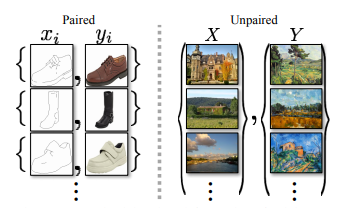
\includegraphics[width=0.5\textwidth]{paired_unpaired.png}
  \caption{Paired training data (left) consists of training examples $\{x_i, y_i\}_{i=1}^N$, where the correspondence between $x_i$ and $y_i$ exists \cite{isola2018imagetoimage}, We instead consider unpaired training data (right), consisting of a source set $\{x_i\}_{i=1}^N (x_i \epsilon X)$ and a target set $\{y_j\}_{j=1}^M (y_j \epsilon Y)$, with no information provided as to which $x_i$ matches which $y_j$.}
  \label{fig:datasetexample}
\end{figure}

\textbf{CycleGan} is ideal for this task as it is specifically designed to be able to learn translation between domains without paired input-output examples (Figure \ref{fig:datasetexample}, right).

\section{Related Work}
%########################################
\subsection{Automatic Image Enhancement}
%########################################
Automatic image enhancement is a well-studied problem in the domains of computer vision, robotics, and signal processing. Classical approaches use hand-crafted filters to enforce local color constancy and improve contrast/lightness rendition \cite{10.1117/1.1636183}. Additionally, prior knowledge or statistical assumptions about a scene (e.g., haze-lines, dark channel prior \cite{berman2019underwater}, etc.) are often utilized for global enhancements such as image deblurring, dehazing \cite{5567108}, etc. Over the last decade, single image enhancement has made remarkable progress due to the advent of deep learning and the availability of large-scale datasets. The contemporary deep CNN-based models provide state-of-the-art performance for problems such as image colorization \cite{zhang2016colorful}, color/contrast adjustment \cite{cheng2016deep}, dehazing \cite{7539399}, etc. These models learn a sequence of non-linear filters from paired training data, which provide much better performance compared to using handcrafted filters.

Moreover, the GAN-based models \cite{goodfellow2014generative} have shown great success for style-transfer and image-to-image translation problems \cite{isola2018imagetoimage}. They employ a two-player min-max game where the ‘generator’ tries to fool the ‘discriminator’ by generating fake images that appear to be sampled from the real distribution. Simultaneously, the discriminator tries to get better at discarding fake images and eventually (in equilibrium) the generator learns to model the underlying distribution. Although such adversarial training can be unstable, several tricks and choices of loss functions are proposed in the literature to mitigate that. For instance, Wasserstein GAN \cite{arjovsky2017wasserstein} improves the training stability by using the earth-mover distance to measure the distance between the data distribution and the model distribution. Energy-based GANs \cite{zhao2017energybased} also improve training stability by modeling the discriminator as an energy function, whereas the LeastSquared GAN \cite{mao2017squares} addresses the vanishing gradients problem by adopting a least-square loss function for the discriminator. On the other hand, conditional GANs \cite{mirza2014conditional} allow constraining the generator to produce samples that follow a pattern or belong to a specific class, which is particularly useful to learn a pixel-to-pixel (Pix2Pix) mapping \cite{isola2018imagetoimage} between an arbitrary input domain (e.g., distorted images) and the desired output domain (e.g., enhanced images).

A major limitation of the above-mentioned models is that they require paired training data, which may not be available or can be difficult to acquire for many practical applications. The two-way GANs (e.g., CycleGAN \cite{zhu2020unpaired}, DualGAN \cite{yi2018dualgan}, etc.) solve this problem by using a ‘cycleconsistency loss’ that allows learning the mutual mappings between two domains from unpaired data. Such models have been effectively used for unpaired learning of perceptual image enhancement \cite{8578758} as well. Furthermore, Ignatov et al. \cite{ignatov2017dslrquality} showed that additional loss-terms for preserving the high-level feature-based content improve the quality of image enhancement using GANs.

\subsection{Improving Underwater Visual Perception}
%########################################
Traditional physics-based methods use the atmospheric dehazing model to estimate the transmission and ambient light in a scene to recover true pixel intensities \cite{cho2018modelassisted, bryson2015truecolor}. Another class of methods design a series of bilateral and trilateral filters to reduce noise and improve global contrast \cite{lu2013underwaterimage, zhang2017underwaterimage}. In recent work, Akkaynaket al. \cite{akkaynak2018arevised} proposed a revised imaging model that accounts for the unique distortions pertaining to underwater light propagation; this contributes to a more accurate color reconstruction and overall a better approximation to the ill-posed underwater image enhancement problem. Nevertheless, these methods require scene depth (or multiple images) and optical waterbody measurements as prior.

On the other hand, several single image enhancement models based on deep adversarial \cite{fabbri2018enhancing, yu2019underwatergan, li2017watergan} and residual learning \cite{liu2019underwaterimage} have reported inspiring results of late. However, they typically use only synthetically distorted images for paired training, which often limit their generalization performance. The extent of large-scale unpaired training on naturally distorted underwater images have not been explored in the literature. Moreover, most existing models fail to ensure fast inference on single-board robotic platforms, which limits their applicability for improving real-time visual perception. We attempt to address these aspects in this paper.

\section{Proposed Model}
%########################################
\subsection{CycleGan Architecture}
%########################################

\begin{figure}[H]
  \centering
  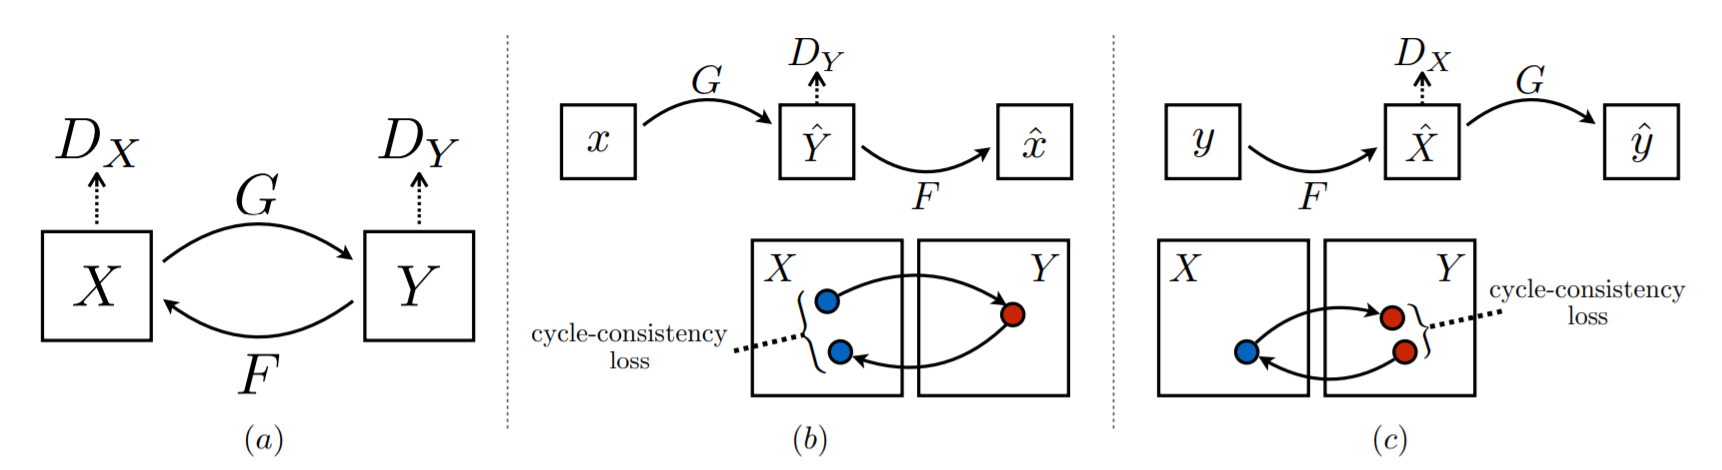
\includegraphics[width=1\textwidth]{cycle_cosistancy.png}
  \caption{(a) Our model contains two mapping functions $G : X → Y$ and $F : Y → X$, and associated adversarial discriminators $D_Y$ and $D_X$. $D_Y$ encourages G to translate X into outputs indistinguishable from domain Y , and vice versa for $DX$ and $F$. To further regularize the mappings, we introduce two cycle consistency losses that capture the intuition that if we translate from one domain to the other and back again we should arrive at where we started: (b) forward cycle-consistency loss: $x → G(x) → F(G(x)) ≈ x$, and (c) backward cycle-consistency loss: $y → F(y) → G(F(y)) ≈ y$}
  \label{fig:cycle_cosistancy}
\end{figure}

\subsection{Generator}
%##########################################
We adopt the architecture for our generative networks from DCGAN \cite{radford2016unsupervised}. The network contains 3 convolution and several residual blocks \cite{he2015deep}, two fractionally-strided convolutions with stride $\frac{1}{2}$, and one convolution that maps features to RGB. We use 6 blocks for 128 × 128 images and 9 blocks for 256×256 and higher-resolution training images. Similar to \cite{johnson2016perceptual}.

We use instance normalization \cite{ulyanov2017instance} and used Leaky ReLU \cite{xu2015empirical} as activation layer. For the last layer, we used hyperbolic tangent as the activation function \cite{6581545}.

\subsection{Discriminator}
%##########################################
The discriminator networks are based on convolutional neural network (CNN)\cite{8308186}. It uses 9 layers of convolutional layer to extract deep features from the image and classify between 2 sets of images.

\section{Objective Function Formulation}
%########################################
Our goal is to learn mapping functions between two domains $X$ and $Y$ given training samples ${x_i}^N_{i=1}$ where ${x_i} \in X$ and ${y_j}^N_{j=1}$
where ${y_j} \in Y$. We denote the data distribution as $x ∼ pdata(x)$ and
$y ∼ pdata(y)$. As illustrated in Figure \ref{fig:cycle_cosistancy} (a), our model includes two mappings $G : X → Y$ and $F : Y → X$. In addition, we introduce two adversarial discriminators $D_X$ and $D_Y$ , where $D_X$ aims to distinguish between images ${x}$ and translated images ${F(y)}$; in the same way, $D_Y$ aims to discriminate between ${y}$ and ${G(x)}$. Our objective contains two types of terms: adversarial losses \cite{NIPS2014_5ca3e9b1} for matching the distribution of generated images to the data distribution in the target domain; and cycle consistency losses to prevent the learned mappings $G$ and $F$ from contradicting each other.

\subsection{Adversarial Loss}
A standard conditional GAN-based model learns a mapping $G : {X, Z} → Y$ , where $X(Y)$ represents the source(desired) domain, and Z denotes random noise. The conditional adversarial loss function\cite{mirza2014conditional} is expressed as:

\begin{equation}
    \label{eq:advloss}
    \mathcal{L}_{GAN}N(G, D_Y , X, Y ) = \mathbb{E}_{X,Y}[\log{D_Y(Y)}] + \mathbb{E}_{X,Y}[\log{1-D(X, G(X,Z))}]
\end{equation}

Here, the generator G tries to minimize $\mathcal{L}_{cGAN}$ while the discriminator $D_Y$ tries to maximize it.

\subsection{Cycle Consistency Loss}
Adversarial training can, in theory, learn mappings $G$ and $F$ that produce outputs identically distributed as target domains $Y$ and $X$ respectively (strictly speaking, this requires $G$ and $F$ to be stochastic functions) \cite{goodfellow2017nips}. However, with large enough capacity, a network can map the same set of input images to any random permutation of images in the target domain, where any of the learned mappings can induce an output distribution that matches the target distribution. Thus, adversarial losses alone cannot guarantee that the learned function can map an individual input $x_i$ to a desired output $y_i$ . To further reduce the space of possible mapping functions, we argue that the learned mapping functions should be cycle-consistent functions should be cycle-consistent: as shown in Figure \ref{fig:cycle_cosistancy} (b), for each image x from domain X, the image translation cycle should be able to bring x back to the original image, i.e., $x → G(x) → F(G(x)) ≈ x$

\begin{equation}
    \label{eq:cycloss}
    \mathcal{L}_{cyc}(G, F) = \mathbb{E}_{x\sim p_{data}(x)}[\left \|F(G(x)) - x\right \|] + \mathbb{E}_{y\sim p_{data}(y)}[\left \|F(G(y)) - y\right \|]
\end{equation}

\subsection{Full Objective}
Our Full objective is:

\begin{equation}
    \label{eq:full_loss}
    \mathcal{L}(G, F, D_X, D_Y) = \mathcal{L}_{GAN}(G, D_Y, X, Y) + \mathcal{L}_{GAN}(F, D_X, Y, X) + \lambda \mathcal{L}_{cyc}(G, F)
\end{equation}

where $\lambda$ controls the relative importance of the two objectives.
We aim to solve:

\begin{equation}
    \label{eq:objective}
    G^*, F^* = arg \min_{G, F} \max_{D_X, D_Y} \mathcal{L}(G, F, D_X, D_Y)
\end{equation}

\section{Training}
To minimize the objective function \ref{eq:objective}, we used Adam optimizer \cite{kingma2017adam} with a batch size of 8. All the networks are trained from ground up with initial learning rate of 0.0002. We keep the same learning rate for first 100 epochs, then linearly decay the learning rate to 0 over the next 100 epochs.

\section{EUVP Dataset}
%########################################
The EUVP dataset contains a large collection of paired and unpaired underwater images of poor and good perceptual quality. We used seven different cameras, which include multiple GoPros \cite{gopro}, Aqua AUV’s uEye cameras \cite{uEye-cameras}, low-light USB cameras \cite{blue-robotics}, and Trident ROV’s HD camera  \cite{openrov}, to capture images for the dataset. The data was collected during oceanic explorations and human-robot cooperative experiments in different locations under various visibility conditions. Additionally, images extracted from a few publicly available $YouTube^{TM}$ videos are included in the dataset. The images are carefully selected to accommodate a wide range of natural variability (e.g., scenes, waterbody types, lighting conditions, etc.) in the data.

The unpaired data is prepared, i.e., good and poor quality images are separated based on visual inspection by six human participants. They inspected several image properties (e.g., color, contrast, and sharpness) and considered whether the scene is visually interpretable, i.e., foreground/objects are identifiable. Hence, the unpaired training endorses the modeling of human perceptual preferences of underwater image quality. On the other hand, the paired data is prepared by following a procedure suggested in \cite{fabbri2018enhancing}. Specifically, a CycleGAN \cite{zhu2020unpaired}-based model is trained on our unpaired data to learn the domain transformation between the good and poor quality images. Subsequently, the good quality images are distorted by the learned model to generate respective pairs; we also augment a set of underwater images from the ImageNet dataset \cite{5206848} and from $Flickr^{TM}$.

\begin{figure}[H]
  \centering
  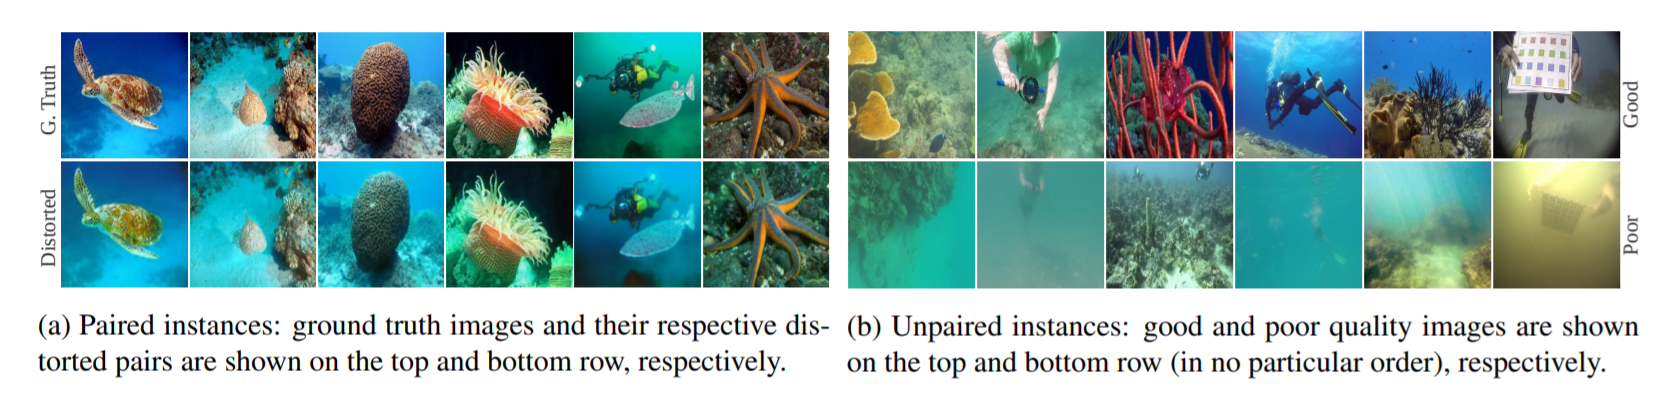
\includegraphics[width=1\textwidth]{euvp_some_example.png}
  \caption{A few sample images from the EUVP dataset are shown.}
  \label{fig:euvpdatasetexample}
\end{figure}

There are over 12K paired and 8K unpaired instances in the EUVP dataset; a few samples are provided in Fig. ~\ref{fig:euvpdatasetexample}. It is to be noted that our focus is to facilitate perceptual image enhancement for boosting robotic scene understanding, not to model the underwater optical degradation process for image restoration, which requires scene depth and waterbody properties.


\section{Experimental Results}
%########################################
\subsection{Qualitative Evaluations}
%########################################
We first qualitatively analyse the output images generated by the model compared to their respective ground truths. As figure \ref{fig:qualitativeanalysis} shows, the bluish hue which is characteristic of underwater images is greatly reduced. Additionally, the model tries to recover the original colour of the objects in the photographs. If trained further the model would be able to learn about the natural colours of the underwater objects and will be able to recreate it much better. Since we only provided unpaired images, the model identified the common artefacts that are present in the A type images but is absent on B type images.

\begin{figure}[H]
  \centering
  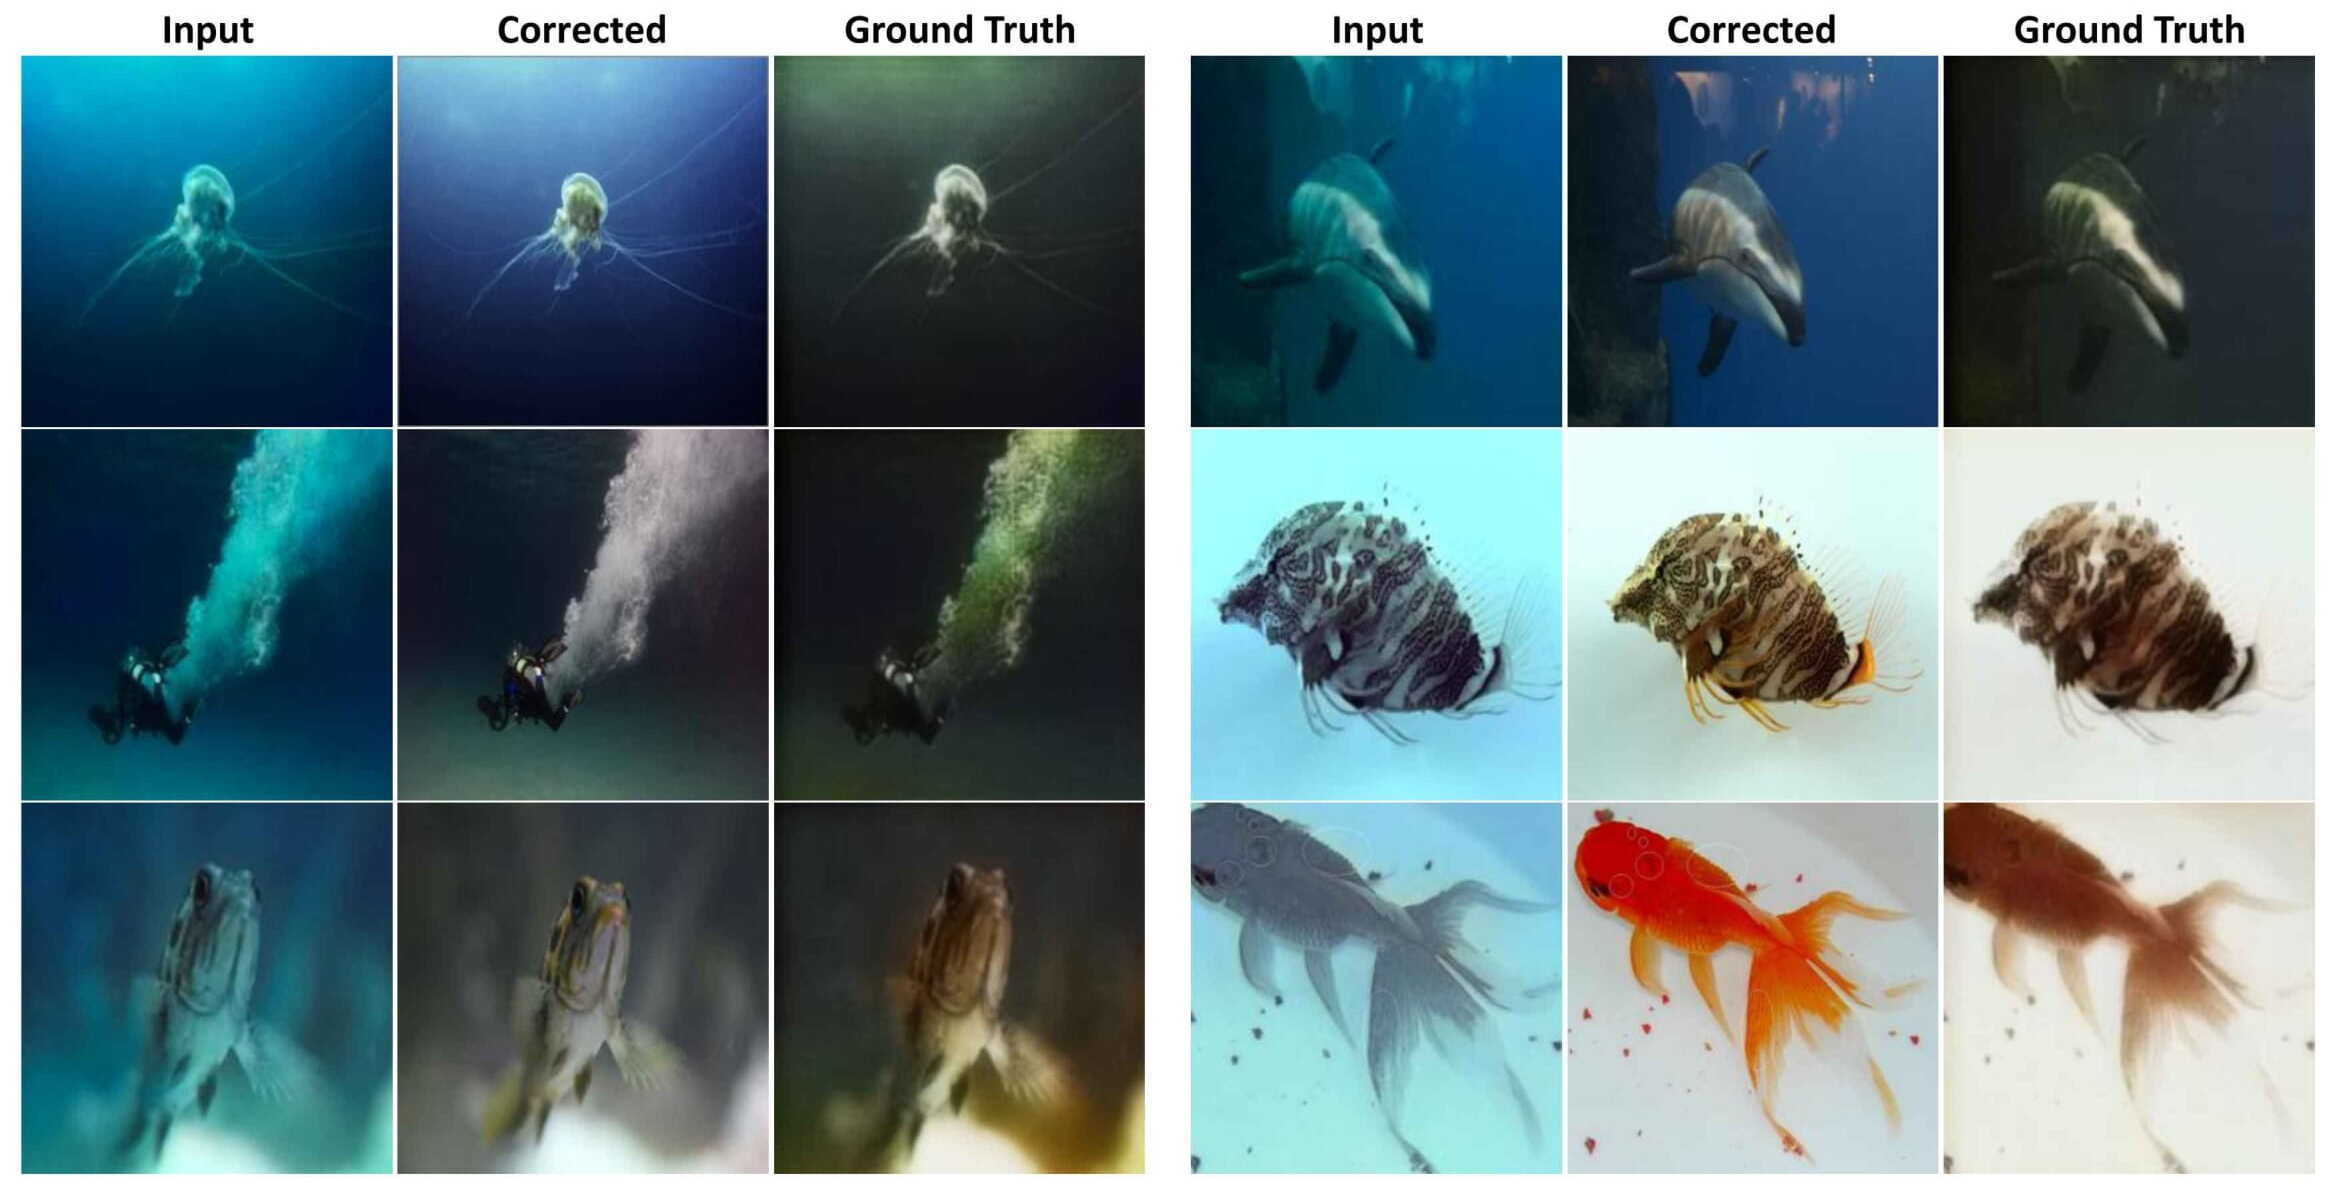
\includegraphics[width=1\textwidth]{qualitative-1.jpg}
  \caption{The bluish hue is rectified and the model tries to regenerate the original colours of the objects.}
  \label{fig:qualitativeanalysis}
\end{figure}

\subsection{Quantitative Evaluation}
%########################################
We consider four standard metrics \cite{ignatov2017dslrquality,8578758,5596999} named Peak Signal-to-Noise Ratio (PSNR), Structural Similarity (SSIM), Entrophy and Underwater Image Quality Metric (UIQM) in order to quantitatively compare CycleGan enhanced images with their respective ground truths.

\subsubsection{Peak Signal-to-Noise Ratio (PSNR)}
%########################################
The PSNR approximates the reconstruction quality of a generated image x compared to its ground truth y based on their Mean Squared Error (MSE) as follows:

\begin{equation}
    \label{eq:psnr}
    PSNR(x, y) = 10\log_{10}[255^{2}/MSE(x,y)]
\end{equation}

\subsubsection{Structural similarity index measurement (SSIM)}
SSIM \cite{wang2004imagequalityassesment} compares the image patches based on three properties: luminance, contrast, and structure. It is defined as follows:

\begin{equation}
    \label{eq:ssim}
    SSIM(x,y)=(\frac{2\mu_{x}\mu_{y} + c_{1}}{\mu_{x}^{2}+\mu_{y}^{2} + c_{1}})(\frac{2\sigma_{xy} + c_{2}}{\sigma_{x}^{2}+\sigma_{y}^{2} + c_{2}})
\end{equation}

In equation \ref{eq:ssim}, $\mu_x\;(\mu_y)$ denotes the mean, and $\sigma_x^2\;(\sigma_y^2)$ is the variance of $x\;(y)$; whereas $\sigma_{xy}$ denotes the cross correlation between $x$ and $y$. Additionally, $c_1 = (255 \times 0.01)^2$ and $c_2 = (255 \times 0.03)^2$ are constants that ensure numeric stability.

\subsubsection{Entropy}
Entropy is a statistical measure of randomness that can be used to characterize the texture of the input image.

The Shannon entropy is defined as:

\begin{equation}
    \label{eq:entrophy}
    S = -\sum(p_k \times \log(p_k))
\end{equation}

In equation \ref{eq:entrophy}, $p_k$ is the frequency/probability of pixels of value $k$.

\subsubsection{Underwater Image Quality Metric (UIQM)}
The \textit{underwater image quality measure (UIQM)} comprises three attribute measures, namely, the \textit{underwater image colorfulness measure (UICM)}, the \textit{underwater image sharpness measure (UISM)}, and the \textit{underwater image contrast measure (UIConM)}. Details of the new measures are presented in this section.

\paragraph{Underwater Image Colorfulness Measure (UICM)}
The UICM deals with the color casting problem. As the depth of the water increases, colors attenuate one by one depending on their wavelength. The color red disappears first due to it possessing the shortest wavelength. As a result, underwater images usually demonstrate a bluish or greenish appearance. Furthermore, limited lighting conditions also causes severe color desaturation in underwater images.

To measure the UICM, we use the two opponent color components related with chrominance, RG and YB as shown in

\begin{equation}
    \label{eq:uicm1}
    RG = R - G
\end{equation}

\begin{equation}
    \label{eq:uicm2}
    YB = \frac{R + G}{2} - B
\end{equation}

Underwater images usually suffer from heavy noise. Therefore, instead of using the regular
statistical values, the asymmetric alpha-trimmed statistical values are used for measuring
underwater image colorfulness. The mean is defined by:

\begin{equation}
    \label{eq:uicm-mean}
    \mu_{\alpha,RG} = \frac{1}{K - T_{\alpha L} - T_{\alpha R}} \sum_{i=T_{\alpha L} + 1}^{K-T_{\alpha R}} Intensity_{RG,i}
\end{equation}

The second-order statistic variance $\sigma^2$ in:
\begin{equation}
    \label{eq:uicm-variance}
    \sigma^2_{\alpha,RG} = \frac{1}{N} \sum_{p=1}^{N}(Intensity_{RG, p} - \mu_{\alpha,RG})^2
\end{equation}

The overall colourfulness metric used for measuring underwater image colourfulness is demonstrated as

\begin{equation}
    \label{eq:uicm-final}
    UICM = -0.0268\sqrt{\mu^2_{\alpha,RG} + \mu^2_{\alpha,YB}} + 0.1586\sqrt{\sigma^2_{\alpha,RG} + \sigma^2_{\alpha,YB}}
\end{equation}

\paragraph{Underwater Image Sharpness Measure (UISM)}
To measure the sharpness on edges, the Sobel edge detector is first applied on each RGB color component. The resultant edge map is then multiplied with the original image to get the grayscale edge map. By doing this, only the pixels on the edges from the original underwater image are preserved. It is known that the enhancement measure estimation (EME) measure is suitable for images with uniform background and shown non-periodic patterns

The UISM is formulated as shown in
\begin{equation}
    \label{eq:uism}
    UISM = \sum_{c=1}^3\lambda_c EME(greyscale, edge_c)
\end{equation}

\begin{equation}
    \label{eq:uism-eme}
    EME = \frac{2}{k_1 k_2}\sum_{l=1}^{k1}\sum_{k=1}^{k2}\log(\frac{I_{max, k, l}}{I_{min, k, l}})
\end{equation}

\paragraph{Underwater Image Contrast Measure (UIConM)}
Contrast has been shown to correspond to underwater visual performance such as stereoscopic acuity [37]. For underwater images, contrast degradation is usually caused by backward scattering

\begin{equation}
    \label{eq:uiconm}
    UIConM = \log{AMEE(Intensity)}
\end{equation}

The $\log{AMEE}$ in

\begin{equation}
    \label{eq:uiconm-logamee}
    \log{AMEE} = \frac{1}{k_1 k_2} \bigotimes \sum_{l=1}^{k_1}\sum_{k=1}^{k_2}\frac{I_{max,k,l} \Theta I_{min,k,l}}{I_{max,k,l} \bigoplus I_{min,k,l}} \times \log(\frac{I_{max,k,l} \Theta I_{min,k,l}}{I_{max,k,l} \bigoplus I_{min,k,l}})
\end{equation}

The overall equation for the \textbf{UIQM} is
\begin{equation}
    \label{eq:uiqm}
    UIQM = c_1 \times UICM + c_2 \times UISM + c_3 \times UIConM
\end{equation}

A generic coefficient set $c_1 = 0.0282$,$c_2 = 0.2953$, and $c_3 = 3.5753$ is used as suggested by \cite{7305804}

\subsubsection{Metrics}

\begin{figure}[H]
  \centering
  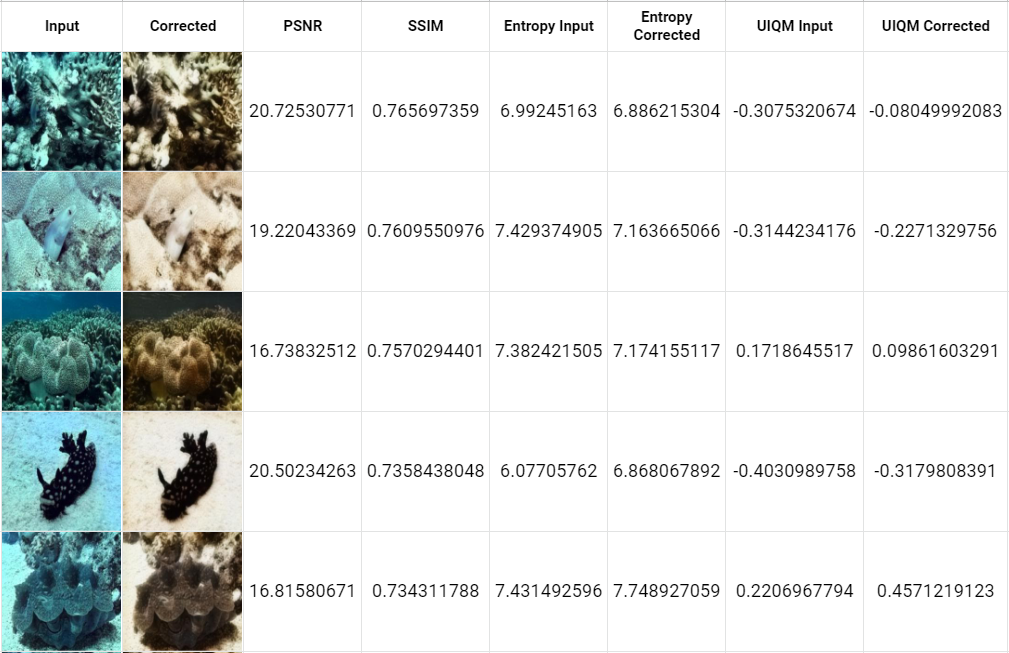
\includegraphics[width=1\textwidth]{quantitative-1.png}
  \caption{Metrics for top 5 enhanced images.}
  \label{fig:quantitativeanalysis}
\end{figure}

\section{Conclusion}
%########################################
In this project we present a simple yet efficient GAN-based model for \textbf{underwater image enhancement}. With the help of \textit{Cycle Generative Adversarial Network (CycleGAN)} the underwater enhancing model can generally and effectively transform underwater images with low visible quality into clean images with richer details and higher visible quality. Our study shows the effectiveness of each module of the proposed model. The proposed model formulates a perceptual loss function by evaluating image quality based on its global color, content, local texture and style information. We performed extensive qualitative and quantitative evaluations. The qualitative and quantitative evaluation results have shown that the proposed model performs as well and often better than the original quality images. We believe that our project demonstrates the potential of CycleGAN for improving the translation quality of underwater images.

\bibliographystyle{plain}
\bibliography{reference}

\end{document}